\documentclass[tikz, border=5pt]{standalone}

\begin{document}
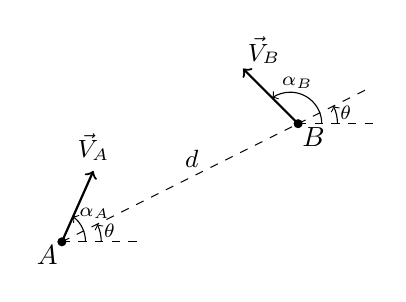
\begin{tikzpicture}

    %% Collision diagram

    % Mass A
    \coordinate (A) at (0,0);
    \draw[fill] (A) circle (0.05) node[below left=-2] {\( A \)};
    \draw[->, thick] (A) -- ++(0.4,0.9) node[above] {\small \( \vec{V}_A \)};

    % Mass B
    \coordinate (B) at (3,1.5);
    \draw[fill] (B) circle (0.05) node[below right=-2] {\( B \)};
    \draw[->, thick] (B) -- ++(-0.7,0.7) node[above right=-2] {\small \( \vec{V}_B \)};

    % Line of separation
    \draw[dashed] (A) -- (B) node[pos=0.55, above] {\small \( d \)};

    % Reference
    \draw[dashed] (A) -- ++(1,0);
    \draw[dashed] (B) -- ++(1,0);
    \draw[dashed] (B) -- ++(0.9,0.45);

    % Angles
    \draw[->] (A) ++(0.5,0) arc (0:27:0.5) node[pos=0.6, right=-2] {\scriptsize \( \theta \)};
    \draw[->] (B) ++(0.5,0) arc (0:27:0.5) node[pos=0.6, right=-2] {\scriptsize \( \theta \)};
    \draw[->] (A) ++(0.3,0) arc (0:54:0.4) node[pos=1.2, right=0.8] {\scriptsize \( \alpha_A \)};
    \draw[->] (B) ++(0.3,0) arc (0:125:0.4) node[above right] {\scriptsize \( \alpha_B \)};

\end{tikzpicture}
\end{document}
